\documentclass[aspectratio=169,12pt,t]{beamer}

% --- Theme: Metropolis (modern, clean) ---
\usetheme[progressbar=frametitle,numbering=fraction,block=fill]{metropolis}

% --- Fira Sans font (install texlive-fonts-extra if missing) ---
\IfFileExists{FiraSans.sty}{\usepackage[sfdefault]{FiraSans}}{}

% --- Light background with warm accent ---
\definecolor{mDarkTeal}{RGB}{35,55,59}
\definecolor{mLightBrown}{RGB}{235,228,216}
\definecolor{mAccent}{RGB}{140,70,20}

\setbeamercolor{normal text}{fg=mDarkTeal,bg=white}
\setbeamercolor{alerted text}{fg=mAccent}
\setbeamercolor{frametitle}{bg=mDarkTeal,fg=white}
\setbeamercolor{progress bar}{fg=mAccent,bg=mLightBrown}
\setbeamercolor{title separator}{fg=mAccent}
\setbeamercolor{progress bar in head/foot}{fg=mAccent,bg=mLightBrown}
\setbeamercolor{progress bar in section page}{fg=mAccent,bg=mLightBrown}

% --- Packages ---
\usepackage[utf8]{inputenc}
\usepackage{amsmath,amssymb,amsthm}
\usepackage{mathrsfs}
\usepackage{tikz}
\usetikzlibrary{arrows.meta,positioning,calc,decorations.pathreplacing,shapes,patterns}
\usepackage{pgfplots}
\pgfplotsset{compat=1.18}

% --- TikZ diagram styles (shared across the series) ---
\tikzset{
  axisln/.style={-{Stealth[length=2.6mm]}, line width=0.8pt, gray!75},
  curveln/.style={line width=1.6pt, line cap=round, line join=round},
  projln/.style={dash pattern=on 2.6pt off 2pt, line width=0.7pt},
  guide/.style={-{Stealth[length=2.6mm,width=2.2mm]}, line width=1.1pt},
}
% point marker with a white halo: \dotpt{color}{(coord)}
\newcommand{\dotpt}[2]{%
  \fill[white] #2 circle (3.6pt);
  \fill[#1] #2 circle (2.4pt);
}
% open point marker: \opendotpt{color}{(coord)}
\newcommand{\opendotpt}[2]{%
  \fill[white] #2 circle (3.6pt);
  \draw[#1, line width=1pt] #2 circle (2.4pt);
}

% --- Semi-transparent white highlight for text on top of background images ---
\usepackage[most]{tcolorbox}

% Inline highlight: \hl{short text}
\newtcbox{\hl}{%
  nobeforeafter, tcbox raise base,
  colback=white, opacityback=0.6,
  colframe=white, opacityframe=0,
  sharp corners, boxsep=2pt, left=3pt, right=3pt, top=2pt, bottom=2pt%
}

% Block highlight: \begin{hlbox} ... \end{hlbox}  (multi-line, paragraphs, itemize)
% Optional argument accepts any tcolorbox key, e.g. [width=0.6\linewidth]
\newtcolorbox{hlbox}[1][]{%
  enhanced, breakable,
  colback=white, opacityback=0.6,
  colframe=white, opacityframe=0,
  boxsep=3pt, left=6pt, right=6pt, top=4pt, bottom=4pt,
  sharp corners,
  {#1}%
}

% --- Custom colors for content types ---
\definecolor{defcolor}{RGB}{25,85,120}
\definecolor{thmcolor}{RGB}{140,35,35}
\definecolor{proofcolor}{RGB}{35,100,50}
\definecolor{excolor}{RGB}{140,75,10}
\definecolor{remcolor}{RGB}{90,90,90}

% --- Beamer blocks for mathematical content types (semi-transparent) ---
\tcbset{hlblockbase/.style={
  enhanced, breakable,
  coltitle=white, fonttitle=\bfseries,
  opacitybacktitle=0.8, opacityback=0.6,
  opacityframe=0,
  sharp corners,
  boxsep=1pt, left=5pt, right=5pt, top=2pt, bottom=2pt,
  toptitle=1pt, bottomtitle=1pt
}}

\newtcolorbox{defblock}[1]{hlblockbase, title={#1},
  colbacktitle=defcolor, colback=defcolor!15, colframe=defcolor}
\newtcolorbox{thmblock}[1]{hlblockbase, title={#1},
  colbacktitle=thmcolor, colback=thmcolor!15, colframe=thmcolor}
\newtcolorbox{proofblock}[1]{hlblockbase, title={#1},
  colbacktitle=proofcolor, colback=proofcolor!15, colframe=proofcolor}
\newtcolorbox{exblock}[1]{hlblockbase, title={#1},
  colbacktitle=excolor, colback=excolor!15, colframe=excolor}
\newtcolorbox{remblock}[1]{hlblockbase, title={#1},
  colbacktitle=remcolor, colback=remcolor!15, colframe=remcolor}

% --- Metadata ---
\title{Chapter 6: The Riemann--Stieltjes Integral}
\subtitle{Section: Properties of the Integral}
\author{Based on Walter Rudin's \emph{Principles of Mathematical Analysis}}
\date{}

\begin{document}

{
\usebackgroundtemplate{%
  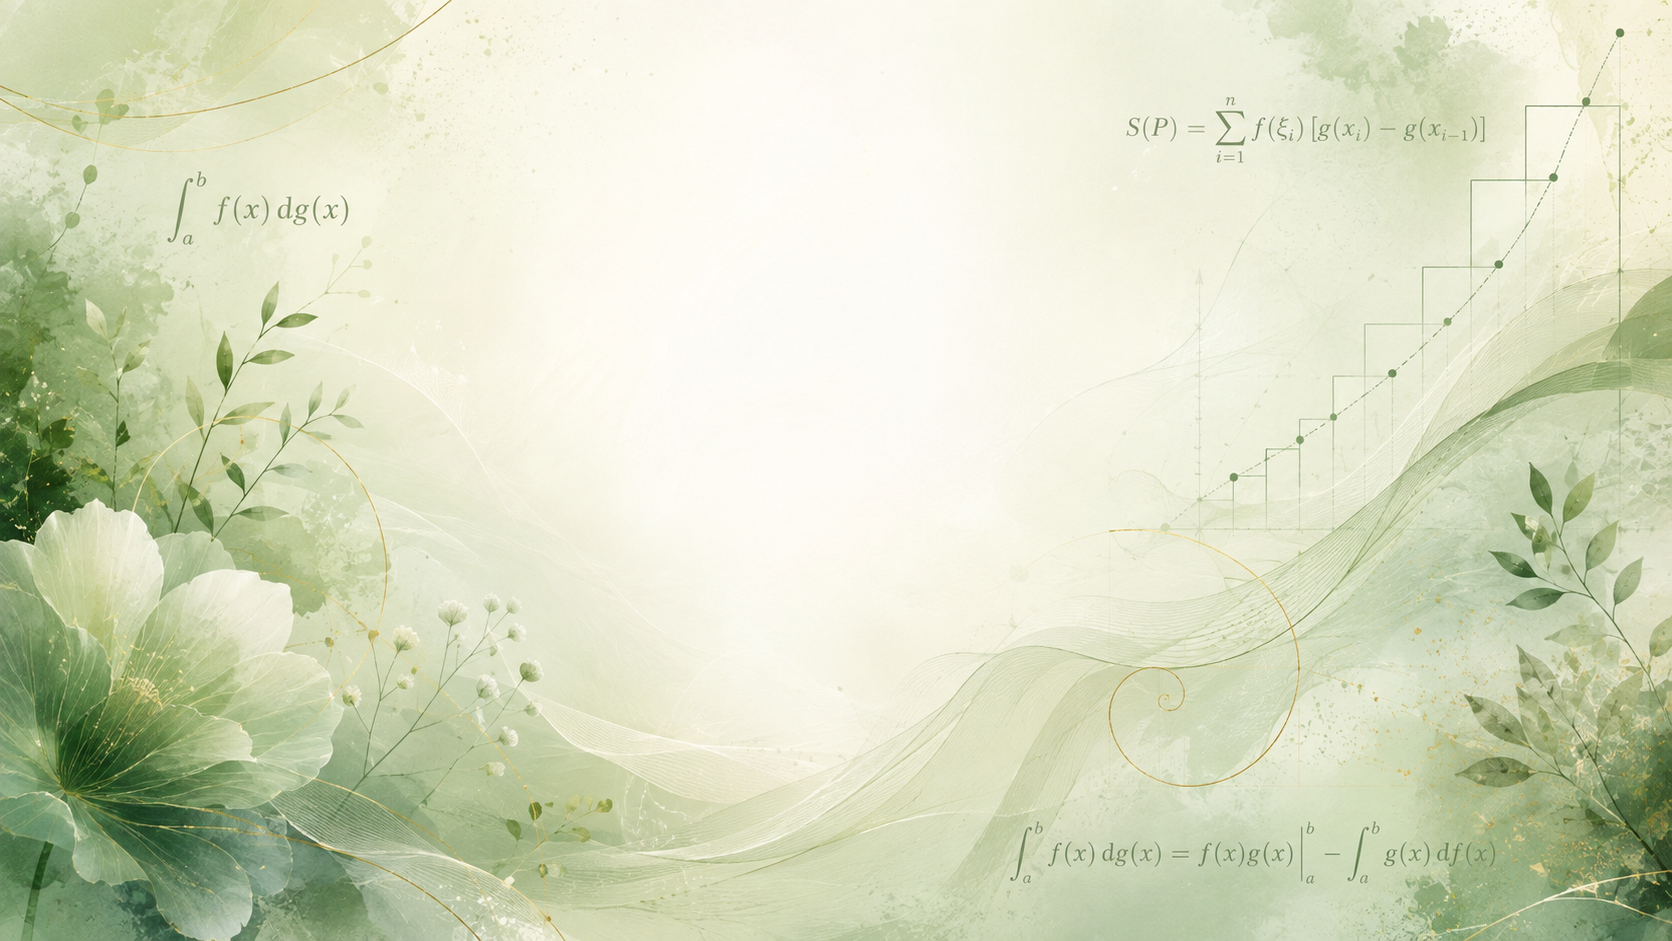
\includegraphics[width=\paperwidth,height=\paperheight,keepaspectratio=false]{chapter_06_bg_00.png}%
}
\begin{frame}[plain]
  \titlepage

  \note{
    Welcome to Chapter 6, Section 2: Properties of the Integral. In the
    previous episode we constructed the Riemann-Stieltjes integral from
    partitions and upper and lower sums, and we proved the Cauchy style
    criterion, Theorem 6.6, which tells us exactly when a bounded
    function is integrable with respect to an increasing weight alpha.
    In this episode we put that criterion to work. First we establish
    the everyday rules of calculus: the integral is linear, it respects
    order, it splits across subintervals, and it obeys a basic size
    bound. Then products and absolute values. And then comes the real
    payoff of the Stieltjes point of view: with a step function as the
    weight, an infinite series literally becomes an integral, and when
    the weight has an integrable derivative, the Stieltjes integral
    collapses to an ordinary Riemann integral. A clean change of
    variable theorem rounds out the toolkit. Let's get started.
  }
\end{frame}
}

{
\usebackgroundtemplate{%
  
\includegraphics[width=\paperwidth,height=\paperheight,keepaspectratio=false]{chapter_06_bg_01.png}%
}
\begin{frame}[c]{Outline}
  \begin{center}
    \tableofcontents
  \end{center}

  \note{
    Here is the plan for this episode. After a short motivation, we
    prove Theorem 6.12, the algebraic properties: linearity in the
    function, monotonicity, splitting the interval at a point, a basic
    size bound, and linearity in the weight. Theorem 6.13 then handles
    products and absolute values, including the integral form of the
    triangle inequality. Next come step functions: Theorems 6.15 and
    6.16 show that integrating against a step function samples the
    function at the jumps, so a convergent series is itself a
    Stieltjes integral. Theorem 6.17 goes the other way: when the
    weight alpha has an integrable derivative, the Stieltjes integral
    reduces to an ordinary Riemann integral. Remark 6.18 ties these
    threads together with a physical example, and Theorem 6.19 gives
    the change of variable formula. We close with a summary and a
    preview of the next episode.
  }
\end{frame}

\section{Motivation}

% --- Build 1/3 ---
\begin{frame}{From Existence to Rules}
  \begin{hlbox}
  \begin{itemize}
    \item Last episode: \alert{when} does $\int_a^b f\,d\alpha$ exist?
      (Theorem 6.6: $U - L < \varepsilon$)
  \end{itemize}
  \end{hlbox}

  \note{
    Let's recall where we stand. The previous episode answered the
    existence question: a bounded function "f" is integrable with
    respect to the increasing weight alpha exactly when, for every
    positive epsilon, some partition brings the upper and lower sums
    within epsilon of each other. That criterion, Theorem 6.6, was the
    workhorse of the whole section. But knowing that an integral
    exists is only half the story.
  }
\end{frame}

% --- Build 2/3 ---
\begin{frame}{From Existence to Rules}
  \begin{hlbox}
  \begin{itemize}
    \item Last episode: \alert{when} does $\int_a^b f\,d\alpha$ exist?
      (Theorem 6.6: $U - L < \varepsilon$)
    \item This episode: \alert{how does the integral behave?}
      Linearity, order, splitting, products, absolute values
  \end{itemize}
  \end{hlbox}

  \note{
    This episode develops the rules for working with integrals: the
    integral of a sum is the sum of the integrals, larger functions
    have larger integrals, an integral over the whole interval splits
    at any intermediate point, and products and absolute values of
    integrable functions remain integrable. These are the facts one
    uses constantly and almost unconsciously in calculus; here each
    one gets an honest proof from the partition machinery.
  }
\end{frame}

% --- Build 3/3 ---
\begin{frame}{From Existence to Rules}
  \begin{hlbox}
  \begin{itemize}
    \item Last episode: \alert{when} does $\int_a^b f\,d\alpha$ exist?
      (Theorem 6.6: $U - L < \varepsilon$)
    \item This episode: \alert{how does the integral behave?}
      Linearity, order, splitting, products, absolute values
    \item The payoff of the Stieltjes viewpoint:
      \begin{align*}
        \text{step weight } \alpha \;&\Rightarrow\;
        \int f\,d\alpha = \sum\nolimits_n c_n f(s_n)
        && \text{(series!)} \\
        \alpha' \in \mathscr{R} \;&\Rightarrow\;
        \int f\,d\alpha = \int f\alpha'\,dx
        && \text{(Riemann!)}
      \end{align*}
  \end{itemize}
  \end{hlbox}

  \note{
    And then the payoff. Two theorems in this episode justify the
    generality of the Stieltjes construction. If the weight alpha is a
    step function that jumps by "c" sub "n" at the point "s" sub "n",
    the integral of "f" becomes the sum of the values "c" sub "n"
    times "f" of "s" sub "n": an infinite series is an integral. If
    instead alpha has an integrable derivative, the Stieltjes integral
    turns into the ordinary Riemann integral of "f" times alpha prime.
    Series and integrals become two faces of one theory. Before
    diving in, let's put our main tool back on the table.
  }
\end{frame}

\begin{frame}{Our Workhorse from Last Time}
  \begin{remblock}{Recall: Theorem 6.6 (the integrability criterion)}
    $f \in \mathscr{R}(\alpha)$ on $[a,b]$ \ $\iff$ \ for every
    $\varepsilon > 0$ there is a partition $P$ with
    \[
      U(P,f,\alpha) - L(P,f,\alpha) < \varepsilon. \tag{13}
    \]
  \end{remblock}

  \vspace{0.3em}
  \begin{remblock}{Recall: Theorem 6.7 (its companions)}
    (a) If (13) holds for $P$, it holds for every \alert{refinement}
    of $P$. \\
    (b) $\sum_i |f(s_i) - f(t_i)|\,\Delta\alpha_i < \varepsilon$ for
    sample points $s_i, t_i \in [x_{i-1},x_i]$. \\
    (c) If $f \in \mathscr{R}(\alpha)$:
    $\bigl|\sum_i f(t_i)\,\Delta\alpha_i - \int_a^b f\,d\alpha\bigr|
    < \varepsilon$.
  \end{remblock}

  \note{
    Almost every proof today runs through these two results, so let's
    restate them. Theorem 6.6, in the top box, converts integrability
    into a concrete task: exhibit one partition whose upper and lower
    sums differ by less than epsilon. Theorem 6.7, in the bottom box,
    adds three practical consequences. Part "a": a good partition
    stays good under refinement. Part "b": once the upper and lower
    sums are within epsilon, the values of "f" at any two sample
    points in each subinterval differ so little that the weighted sum
    of those differences stays below epsilon. Part "c": Riemann
    Stieltjes sums built from arbitrary sample points approximate the
    integral to within epsilon. With the toolkit ready, here is the
    first batch of properties.
  }
\end{frame}

}

{
\usebackgroundtemplate{%
  
\includegraphics[width=\paperwidth,height=\paperheight,keepaspectratio=false]{chapter_06_bg_02.png}%
}
\section{Algebraic Properties}

\begin{frame}{Theorem 6.12(a): Linearity in the Function}
  \begin{thmblock}{Theorem 6.12(a)}
    If $f_1 \in \mathscr{R}(\alpha)$ and $f_2 \in \mathscr{R}(\alpha)$
    on $[a,b]$, then $f_1 + f_2 \in \mathscr{R}(\alpha)$,
    \ $cf \in \mathscr{R}(\alpha)$ for every constant $c$, and
    \[
      \int_a^b (f_1 + f_2)\,d\alpha
      = \int_a^b f_1\,d\alpha + \int_a^b f_2\,d\alpha,
      \qquad
      \int_a^b cf\,d\alpha = c\int_a^b f\,d\alpha.
    \]
  \end{thmblock}

  \vspace{0.3em}
  \hl{\textbf{Key idea:} integration is a \alert{linear} operation on
  $\mathscr{R}(\alpha)$.}

  \note{
    Theorem 6.12 is a package of five basic properties; we take them
    one at a time. Part "a" is linearity in the function. If "f" sub 1
    and "f" sub 2 are both integrable with respect to alpha, then so
    is their sum, and so is any constant multiple, and the integral
    acts linearly: the integral of the sum is the sum of the
    integrals, and constants pull out. In modern language, the
    integrable functions form a vector space, and the integral is a
    linear functional on it. This is the property we will prove in
    detail; it is a perfect showcase for the Theorem 6.6 criterion.
  }
\end{frame}

\begin{frame}{Theorem 6.12(b): Monotonicity}
  \begin{thmblock}{Theorem 6.12(b)}
    If $f_1(x) \leq f_2(x)$ on $[a,b]$, then
    \[
      \int_a^b f_1\,d\alpha \;\leq\; \int_a^b f_2\,d\alpha.
    \]
  \end{thmblock}

  \begin{center}
  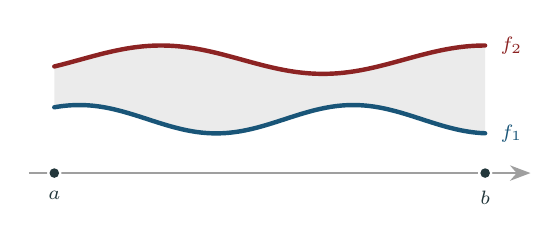
\begin{tikzpicture}[scale=0.72, declare function={
      fone(\x) = 0.95 + 0.25*sin(1.3*\x r + 1 r);
      ftwo(\x) = 2.0 + 0.25*sin(1.1*\x r - 0.5 r);}]
    % gap between the curves
    \fill[remcolor!12]
      plot[domain=0:7.6, samples=60, smooth] (\x,{ftwo(\x)})
      -- plot[domain=7.6:0, samples=60, smooth] (\x,{fone(\x)})
      -- cycle;
    \draw[axisln] (-0.45,0) -- (8.4,0);
    \draw[curveln, defcolor]
      plot[domain=0:7.6, samples=80, smooth] (\x,{fone(\x)});
    \draw[curveln, thmcolor]
      plot[domain=0:7.6, samples=80, smooth] (\x,{ftwo(\x)});
    \node[defcolor, font=\scriptsize, right] at (7.7,{fone(7.6)})
      {$f_1$};
    \node[thmcolor, font=\scriptsize, right] at (7.7,{ftwo(7.6)})
      {$f_2$};
    \foreach \x/\lab in {0/{a}, 7.6/{b}} {
      \dotpt{mDarkTeal}{(\x,0)}
      \node[mDarkTeal, font=\scriptsize, below=3pt] at (\x,0) {$\lab$};
    }
  \end{tikzpicture}
  \end{center}

  \vspace{-0.2em}
  \hl{\textbf{Key idea:} the integral \alert{respects order}.}

  \note{
    Part "b" says the integral respects order. In the picture, the
    red graph of "f" sub 2 runs everywhere above the blue graph of
    "f" sub 1, and the gray band is the gap between them; the claim
    is that the integral of the upper function is at least the
    integral of the lower one. The reason is visible at the level of
    sums. On each subinterval, the supremum of "f" sub 1 is at most
    the supremum of "f" sub 2, and since the increments delta alpha
    sub "i" are nonnegative, every upper sum of "f" sub 1 is at most
    the corresponding upper sum of "f" sub 2. Taking the infimum
    over all partitions passes the inequality to the integrals.
    Monotonicity is the source of virtually every estimate involving
    integrals.
  }
\end{frame}

\begin{frame}{Theorem 6.12(c): Splitting the Interval}
  \begin{thmblock}{Theorem 6.12(c)}
    If $f \in \mathscr{R}(\alpha)$ on $[a,b]$ and $a < c < b$, then
    $f \in \mathscr{R}(\alpha)$ on $[a,c]$ and on $[c,b]$, and
    \[
      \int_a^c f\,d\alpha + \int_c^b f\,d\alpha = \int_a^b f\,d\alpha.
    \]
  \end{thmblock}

  \begin{center}
  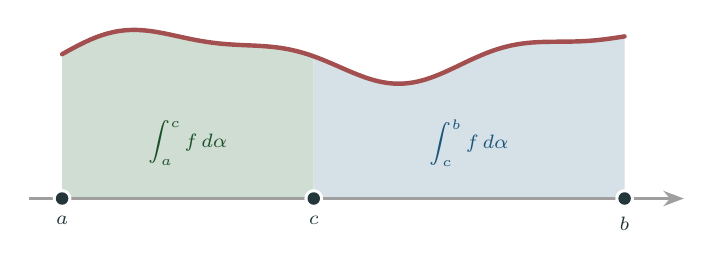
\begin{tikzpicture}[scale=0.94, declare function={
      fc(\x) = 1.95 + 0.30*sin(1.05*\x r) + 0.10*sin(2.4*\x r);}]
    % areas under the curve, split at c
    \fill[proofcolor!22]
      plot[domain=0:3.4, samples=40, smooth] (\x,{fc(\x)})
      -- (3.4,0) -- (0,0) -- cycle;
    \fill[defcolor!18]
      plot[domain=3.4:7.6, samples=40, smooth] (\x,{fc(\x)})
      -- (7.6,0) -- (3.4,0) -- cycle;
    % axis
    \draw[axisln] (-0.45,0) -- (8.4,0);
    % curve on top
    \draw[curveln, thmcolor!80]
      plot[domain=0:7.6, samples=80, smooth] (\x,{fc(\x)});
    % partition points
    \foreach \x/\lab in {0/{a}, 3.4/{c}, 7.6/{b}} {
      \dotpt{mDarkTeal}{(\x,0)}
      \node[mDarkTeal, font=\scriptsize, below=3pt] at (\x,0) {$\lab$};
    }
    % region labels
    \node[proofcolor!80!black, font=\scriptsize] at (1.7,0.75)
      {$\displaystyle\int_a^c f\,d\alpha$};
    \node[defcolor, font=\scriptsize] at (5.5,0.75)
      {$\displaystyle\int_c^b f\,d\alpha$};
  \end{tikzpicture}
  \end{center}

  \note{
    Part "c" is additivity over subintervals. If "f" is integrable on
    the whole interval from "a" to "b", and "c" is any point strictly
    between them, then "f" is integrable on each half, and the two
    pieces add up to the whole. The picture shows the graph of "f"
    with the interval split at "c": the green region is the integral
    from "a" to "c", the blue region is the integral from "c" to "b",
    and together they make up the integral over the full interval.
    The proof device, which we return to once part "a" is proved, is
    to work only with partitions that contain the point "c". Note that
    the splitting goes both ways: it also lets us build integrals over
    long intervals out of integrals over short ones.
  }
\end{frame}

\begin{frame}{Theorem 6.12(d): The Basic Size Bound}
  \begin{thmblock}{Theorem 6.12(d)}
    If $f \in \mathscr{R}(\alpha)$ on $[a,b]$ and $|f(x)| \leq M$ on
    $[a,b]$, then
    \[
      \left|\int_a^b f\,d\alpha\right| \;\leq\; M\,[\alpha(b) - \alpha(a)].
    \]
  \end{thmblock}

  \begin{center}
  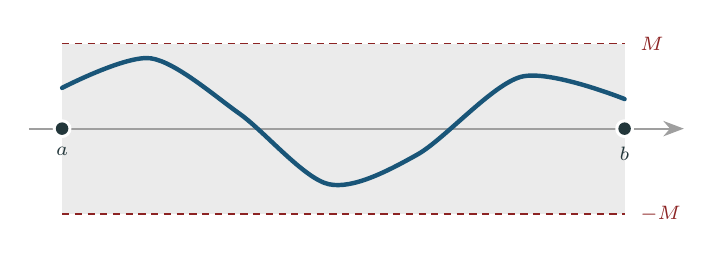
\begin{tikzpicture}[scale=0.94]
    % envelope band
    \fill[remcolor!12] (0,-1.15) rectangle (7.6,1.15);
    \draw[axisln] (-0.45,0) -- (8.4,0);
    \draw[projln, thmcolor] (0,1.15) -- (7.6,1.15)
      node[right=2pt, font=\scriptsize] {$M$};
    \draw[projln, thmcolor] (0,-1.15) -- (7.6,-1.15)
      node[right=2pt, font=\scriptsize] {$-M$};
    \draw[curveln, defcolor] plot[smooth] coordinates
      {(0,0.55) (1.2,0.95) (2.4,0.2) (3.6,-0.75) (4.8,-0.35)
       (6.2,0.7) (7.6,0.4)};
    \foreach \x/\lab in {0/{a}, 7.6/{b}} {
      \dotpt{mDarkTeal}{(\x,0)}
      \node[mDarkTeal, font=\scriptsize, below=3pt] at (\x,0) {$\lab$};
    }
  \end{tikzpicture}
  \end{center}

  \note{
    Part "d" is the basic size estimate. If the values of "f" never
    exceed "M" in absolute value, then the integral never exceeds "M"
    times the total rise of the weight, alpha of "b" minus alpha of
    "a". In the picture, the blue graph of "f" stays inside the gray
    band between the dashed lines at heights "M" and minus "M", and
    the integral is correspondingly trapped. For the ordinary Riemann
    integral, where alpha of "x" equals "x", the bound reads "M"
    times the length of the interval: height times width. This
    innocent estimate will be used again and again, starting with
    Theorem 6.16 later in this episode.
  }
\end{frame}

\begin{frame}{Theorem 6.12(e): Linearity in the Weight}
  \begin{thmblock}{Theorem 6.12(e)}
    If $f \in \mathscr{R}(\alpha_1)$ and $f \in \mathscr{R}(\alpha_2)$,
    then $f \in \mathscr{R}(\alpha_1 + \alpha_2)$ and
    \[
      \int_a^b f\,d(\alpha_1 + \alpha_2)
      = \int_a^b f\,d\alpha_1 + \int_a^b f\,d\alpha_2\,;
    \]
    if $f \in \mathscr{R}(\alpha)$ and $c > 0$ is constant, then
    $f \in \mathscr{R}(c\alpha)$ and
    \[
      \int_a^b f\,d(c\alpha) = c\int_a^b f\,d\alpha.
    \]
  \end{thmblock}

  \vspace{0.3em}
  \hl{\textbf{Key idea:} the integral is linear in the function
  $f$ \emph{and} the weight $\alpha$.}

  \note{
    Part "e" is the mirror image of part "a": linearity in the weight.
    If "f" is integrable with respect to two increasing weights, it is
    integrable with respect to their sum, and the integrals add;
    positive constants scale the same way. The mechanism is
    transparent at the level of sums, because the increment of alpha
    sub 1 plus alpha sub 2 over a subinterval is the sum of the two
    increments. So the Stieltjes integral is linear in both of its
    arguments, the function and the weight. Keep part "e" in mind: it
    is exactly what lets us split a step function weight into a
    finite part plus a small tail in Theorem 6.16. Now let's prove
    part "a" carefully.
  }
\end{frame}

\begin{frame}{Proof of Theorem 6.12(a) --- Step 1: The Key Inequality}
  \begin{proofblock}{Step 1: Sums of functions vs.\ sums of sums}
    \small
    Let $f = f_1 + f_2$. For \emph{any} partition $P$ of $[a,b]$:
    \begin{equation}
      L(P,f_1,\alpha) + L(P,f_2,\alpha) \;\leq\; L(P,f,\alpha)
      \;\leq\; U(P,f,\alpha) \;\leq\; U(P,f_1,\alpha) + U(P,f_2,\alpha).
      \tag{20}
    \end{equation}
  \end{proofblock}

  \vspace{0.3em}
  \begin{hlbox}
  \textbf{Why:} on each subinterval,
  $\sup\,(f_1 + f_2) \leq \sup f_1 + \sup f_2$ \ and \
  $\inf\,(f_1 + f_2) \geq \inf f_1 + \inf f_2$.
  \end{hlbox}

  \note{
    Write "f" for the sum of "f" sub 1 and "f" sub 2. Inequality 20 on
    the slide compares the sums for "f" with the sums for the two
    summands, for one fixed partition. The reason is at the bottom.
    On any subinterval, the supremum of a sum is at most the sum of
    the suprema: the two functions need not achieve their largest
    values at the same point, so adding first and then taking the sup
    can only lose. Dually, the infimum of the sum is at least the sum
    of the infima. Multiplying by the nonnegative increments delta
    alpha sub "i" and adding over the subintervals gives 20. Notice
    the outer terms sandwich the sums for "f"; now we spring the trap.
  }
\end{frame}

\begin{frame}{Proof of Theorem 6.12(a) --- Step 2: $f_1 + f_2$ Is Integrable}
  \begin{proofblock}{Step 2: Apply the criterion}
    Given $\varepsilon > 0$, choose partitions $P_j$ $(j = 1,2)$ with
    \[
      U(P_j, f_j, \alpha) - L(P_j, f_j, \alpha) < \varepsilon.
    \]
    These persist for the \alert{common refinement} $P$ of $P_1, P_2$.
    Then (20) gives
    \[
      U(P,f,\alpha) - L(P,f,\alpha) < 2\varepsilon
      \qquad\Longrightarrow\qquad f \in \mathscr{R}(\alpha).
    \]
  \end{proofblock}

  \vspace{0.3em}
  \begin{hlbox}
  \textbf{Technique:} one partition must work for \alert{both}
  functions --- take the common refinement.
  \end{hlbox}

  \note{
    Integrability first. Let epsilon be positive. Since "f" sub 1 and
    "f" sub 2 are integrable, Theorem 6.6 hands us a good partition
    for each: one with upper minus lower sum below epsilon for "f"
    sub 1, another for "f" sub 2. These are different partitions, so
    we pass to their common refinement "P"; by Theorem 6.7 part "a",
    both inequalities survive refinement. Now read inequality 20 for
    this single partition "P": the outer terms bound the gap between
    the upper and lower sums of "f" by the two gaps for "f" sub 1 and
    "f" sub 2 added together, hence by less than 2 epsilon. Since epsilon was arbitrary,
    Theorem 6.6 says the sum is integrable. Next, the value of its
    integral.
  }
\end{frame}

\begin{frame}{Proof of Theorem 6.12(a) --- Step 3: The Value from Above}
  \begin{proofblock}{Step 3: Compare with the sum of the integrals}
    \small
    With this same $P$,
    \[
      U(P, f_j, \alpha) < \int f_j\,d\alpha + \varepsilon
      \qquad (j = 1,2);
    \]
    hence (20) implies
    \[
      \int f\,d\alpha \;\leq\; U(P,f,\alpha)
      \;<\; \int f_1\,d\alpha + \int f_2\,d\alpha + 2\varepsilon.
    \]
    Since $\varepsilon$ was arbitrary,
    \begin{equation}
      \int f\,d\alpha \;\leq\; \int f_1\,d\alpha + \int f_2\,d\alpha.
      \tag{21}
    \end{equation}
  \end{proofblock}

  \note{
    Now we pin down the value. For the same partition "P", the upper
    sum of each "f" sub "j" lies within epsilon of its integral;
    that is because the gap between its upper and lower sums is below
    epsilon and the integral sits inside that gap. The integral of
    "f" is at most its upper sum, which by inequality 20 is at most
    the two upper sums added, which is less than the sum of the two
    integrals plus 2 epsilon. Letting epsilon shrink to zero yields
    inequality 21: the integral of the sum is at most the sum of the
    integrals. That is only one direction; the lower sums give the
    other, by exactly the same reasoning.
  }
\end{frame}

\begin{frame}{Proof of Theorem 6.12(a) --- Step 4: The Value from Below}
  \begin{proofblock}{Step 4: Run Step 3 with \emph{lower} sums}
    \small
    With the same $P$: \ $L(P, f_j, \alpha) > \int f_j\,d\alpha
    - \varepsilon$ \ $(j = 1,2)$. \ The \alert{left} half of (20)
    then gives
    \[
      \int f\,d\alpha \;\geq\; L(P,f,\alpha)
      \;\geq\; L(P,f_1,\alpha) + L(P,f_2,\alpha)
      \;>\; \int f_1\,d\alpha + \int f_2\,d\alpha - 2\varepsilon.
    \]
    Since $\varepsilon$ was arbitrary, this \alert{reverses} (21):
    \[
      \boxed{\displaystyle\int (f_1+f_2)\,d\alpha
      = \int f_1\,d\alpha + \int f_2\,d\alpha}
      \qquad \text{\qed}
    \]
  \end{proofblock}

  \vspace{0.3em}
  \hl{\textbf{Technique:} (20) is a \alert{two-sided} sandwich --- use
  each half once.}

  \note{
    Step 4 is Step 3 in a mirror. Notice that Step 3 used only the
    right hand half of inequality 20, the half about upper sums. The
    left hand half, about lower sums, is still sitting there unused,
    and it delivers the opposite inequality. For the same partition
    "P", each lower sum of "f" sub "j" now sits within epsilon of its
    integral, this time from below. The integral of "f" is at least
    its lower sum, which by 20 is at least the two lower sums added,
    which beats the sum of the two integrals minus 2 epsilon. Letting
    epsilon shrink reverses 21, and two opposite inequalities mean
    equality, so the boxed formula is proved. One temptation worth
    resisting here: applying 21 to minus "f" sub 1 and minus "f" sub 2
    looks quicker, but it quietly uses the constant multiple rule,
    which is part of what we are still proving. The lower sums keep
    the argument honest.
  }
\end{frame}

\begin{frame}{Theorem 6.12: The Remaining Parts}
  \begin{remblock}{Rudin: ``The proofs are so similar that we omit the
    details''}
    \begin{itemize}
      \item the $cf$ half of (a), and (b), (d), (e): run the
        \alert{same pattern} --- compare sums, apply Theorem 6.6,
        squeeze with $\varepsilon$
      \item (c): the point is to restrict to partitions that
        \alert{contain the point $c$} (pass to refinements!);
        each such $P$ splits into a partition of $[a,c]$ and one of
        $[c,b]$
    \end{itemize}
  \end{remblock}

  \note{
    Rudin proves the additivity half of part "a" and leaves the rest
    as variations on the theme, including the constant multiple rule
    that we were careful not to lean on a moment ago. One of the
    omissions deserves attention, though, the mechanism behind
    part "c". When approximating the integral over the whole
    interval, we may restrict attention to partitions that contain
    the point "c": adding "c" to any partition is a refinement, which
    only improves the sums. And a partition containing "c" splits
    cleanly into a partition of the left half and a partition of the
    right half, with the sums adding accordingly. That is how
    integrability passes to the two subintervals and why the two
    integrals add up to the whole. With the algebraic rules in hand,
    we turn to products and absolute values.
  }
\end{frame}

}

{
\usebackgroundtemplate{%
  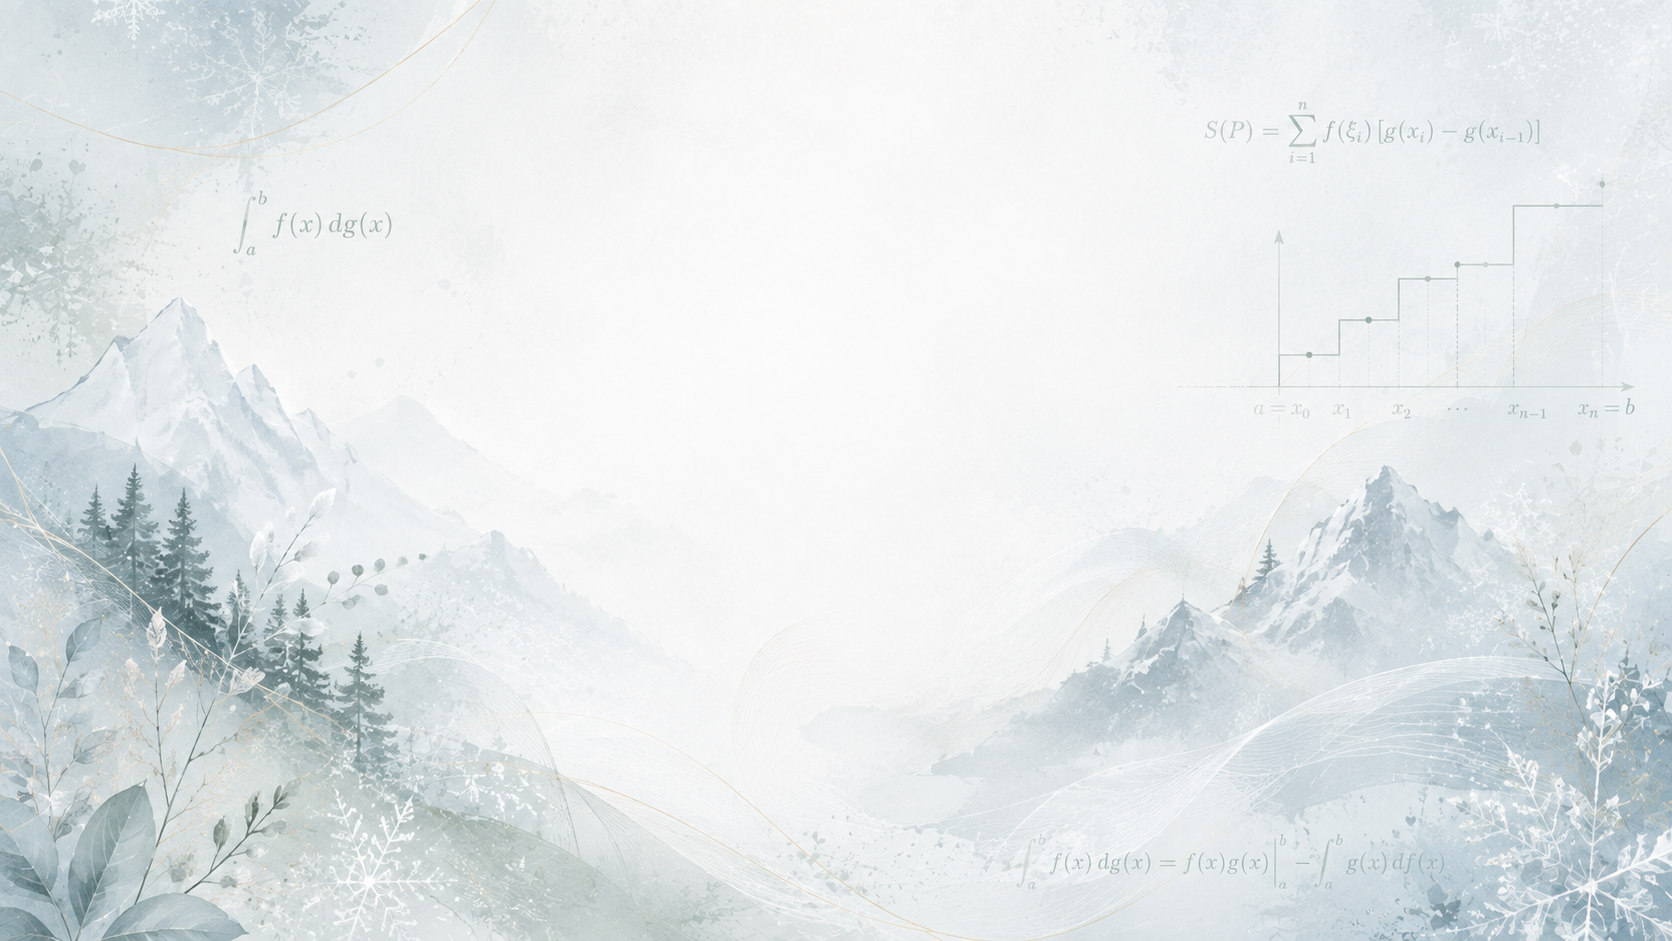
\includegraphics[width=\paperwidth,height=\paperheight,keepaspectratio=false]{chapter_06_bg_03.png}%
}
\section{Products and Absolute Values}

% --- Build 1/2 ---
\begin{frame}{Theorem 6.13: Products and Absolute Values}
  \begin{thmblock}{Theorem 6.13}
    If $f \in \mathscr{R}(\alpha)$ and $g \in \mathscr{R}(\alpha)$ on
    $[a,b]$, then
    \begin{enumerate}
      \item[(a)] $fg \in \mathscr{R}(\alpha)$;
    \end{enumerate}
  \end{thmblock}

  \note{
    Theorem 6.13 adds two closure properties. Part "a": the product of
    two integrable functions is integrable. Note carefully what is
    not claimed: there is no formula expressing the integral of "f"
    times "g" through the integrals of "f" and "g" separately, and
    indeed no such formula can exist. The claim is purely that
    integrability survives multiplication. The proof will be a
    striking application of the composition theorem from last
    episode, Theorem 6.11, combined with an algebraic identity.
    Part "b" is next.
  }
\end{frame}

% --- Build 2/2 ---
\begin{frame}{Theorem 6.13: Products and Absolute Values}
  \begin{thmblock}{Theorem 6.13}
    If $f \in \mathscr{R}(\alpha)$ and $g \in \mathscr{R}(\alpha)$ on
    $[a,b]$, then
    \begin{enumerate}
      \item[(a)] $fg \in \mathscr{R}(\alpha)$;
      \item[(b)] $|f| \in \mathscr{R}(\alpha)$ \ and \
        $\displaystyle\left|\int_a^b f\,d\alpha\right|
        \leq \int_a^b |f|\,d\alpha.$
    \end{enumerate}
  \end{thmblock}

  \vspace{0.3em}
  \begin{hlbox}
  \textbf{Key idea:} (b) is the \alert{triangle inequality for
  integrals} --- an integral is a limit of sums, and sums obey
  $|x + y| \leq |x| + |y|$.
  \end{hlbox}

  \note{
    Part "b": the absolute value of an integrable function is
    integrable, and the absolute value of the integral is at most the
    integral of the absolute value. This is the integral form of the
    triangle inequality, and it is easy to believe: an integral is
    built from sums, and for sums the absolute value of a sum is at
    most the sum of absolute values. Both parts flow from one source,
    Theorem 6.11 on compositions, which said that a continuous
    function of an integrable function is integrable. Let's see how.
  }
\end{frame}

\begin{frame}{Proof of Theorem 6.13(a) --- Step 1: Squares}
  \begin{remblock}{Recall: Theorem 6.11 (composition)}
    If $f \in \mathscr{R}(\alpha)$, $m \leq f \leq M$, and $\phi$ is
    continuous on $[m,M]$,\\
    then $h = \phi \circ f \in \mathscr{R}(\alpha)$.
  \end{remblock}

  \vspace{0.3em}
  \begin{proofblock}{Step 1: $f \in \mathscr{R}(\alpha) \Rightarrow
    f^2 \in \mathscr{R}(\alpha)$}
    Take $\phi(t) = t^2$ (continuous!). Theorem 6.11 gives
    \[
      f \in \mathscr{R}(\alpha) \;\Longrightarrow\;
      f^2 = \phi \circ f \in \mathscr{R}(\alpha).
    \]
  \end{proofblock}

  \note{
    First, squares. Recall Theorem 6.11 from the previous episode, in
    the gray box: composing an integrable function on the inside with
    a continuous function on the outside produces an integrable
    function. The function phi of "t" equals "t" squared is
    continuous on any bounded interval, so if "f" is integrable, so
    is its square. That alone does not give products; for that we
    need to write a product in terms of squares, and there is a
    classical identity that does exactly this.
  }
\end{frame}

\begin{frame}{Proof of Theorem 6.13(a) --- Step 2: The Polarization Trick}
  \begin{proofblock}{Step 2: Products from squares}
    \[
      4fg = (f+g)^2 - (f-g)^2.
    \]
    \begin{itemize}
      \item $f + g,\ f - g \in \mathscr{R}(\alpha)$ \hfill
        [Theorem 6.12(a)]
      \item $(f+g)^2,\ (f-g)^2 \in \mathscr{R}(\alpha)$ \hfill [Step 1]
      \item $4fg \in \mathscr{R}(\alpha)$, hence
        $fg \in \mathscr{R}(\alpha)$ \hfill [Theorem 6.12(a)]
    \end{itemize}
    \qed
  \end{proofblock}

  \vspace{0.3em}
  \begin{hlbox}
  \textbf{Technique:} the \alert{polarization identity}:\\
  recover a product from squares of sums and differences.
  \end{hlbox}

  \note{
    Expand both squares and watch the cancellation: "f" squared and
    "g" squared appear in each expansion and cancel in the
    difference, while the cross terms reinforce, leaving 4 times "f"
    times "g". Now read the chain on the slide. The sum and the
    difference of "f" and "g" are integrable by linearity. Their
    squares are integrable by Step 1. The difference of those squares
    is integrable by linearity again, and dividing by 4 keeps
    integrability. So the product is integrable, exactly as claimed.
    This identity is called polarization, and it reappears throughout
    analysis, most famously connecting norms and inner products.
    Next, absolute values.
  }
\end{frame}

\begin{frame}{Proof of Theorem 6.13(b) --- Step 1: $|f|$ Is Integrable}
  \begin{proofblock}{Step 1: Compose with $\phi(t) = |t|$}
    The absolute value function is continuous, so Theorem 6.11 gives
    \[
      f \in \mathscr{R}(\alpha) \;\Longrightarrow\;
      |f| = \phi \circ f \in \mathscr{R}(\alpha).
    \]
  \end{proofblock}

  \vspace{0.3em}
  \hl{\textbf{Same trick, different $\phi$:} yesterday $t^2$, today $|t|$.}

  \note{
    The first half of part "b" is Theorem 6.11 again with a different
    outer function: phi of "t" equals the absolute value of "t". This
    phi is continuous on the whole line, even though it fails to be
    differentiable at zero; continuity is all that Theorem 6.11
    requires. So the absolute value of an integrable function is
    integrable. It remains to prove the inequality, and Rudin does it
    with a small gem of an argument: one well-chosen sign.
  }
\end{frame}

\begin{frame}{Proof of Theorem 6.13(b) --- Step 2: One Well-Chosen Sign}
  \begin{proofblock}{Step 2: Choose $c = \pm 1$}
    Pick $c = \pm 1$ so that \ $c \displaystyle\int f\,d\alpha \geq 0$.
    Then
    \[
      \left|\int f\,d\alpha\right|
      = c\int f\,d\alpha
      = \int cf\,d\alpha
      \;\leq\; \int |f|\,d\alpha,
    \]
    since $cf \leq |f|$. \hfill [6.12(a) for the middle step,
    6.12(b) for the last] \qed
  \end{proofblock}

  \vspace{0.3em}
  \begin{hlbox}
  \textbf{Technique:} a single sign choice replaces a two-case
  argument.
  \end{hlbox}

  \note{
    Here is the argument. The integral of "f" is some real number,
    possibly negative. Choose the sign "c", either plus 1 or minus 1,
    that makes "c" times the integral nonnegative; then "c" times the
    integral is exactly the absolute value of the integral. Now push
    "c" inside the integral, which is legitimate by linearity, part
    "a" of Theorem 6.12. Finally, "c" times "f" is at most the
    absolute value of "f" pointwise, whatever the sign, so
    monotonicity, part "b", bounds the integral of "c" "f" by the
    integral of the absolute value. Done. Notice the economy of this,
    which is the point of the line at the bottom of the slide: the
    obvious route would split into two cases according to whether the
    integral is positive or negative, and the single letter "c"
    absorbs both cases at once. This sign trick returns later in this
    chapter, in a more sophisticated form, when we integrate vector
    valued functions. Now for the most
    striking theorems of this episode: step function weights.
  }
\end{frame}

}

{
\usebackgroundtemplate{%
  
\includegraphics[width=\paperwidth,height=\paperheight,keepaspectratio=false]{chapter_06_bg_04.png}%
}
\section{Step Functions: Series as Integrals}

\begin{frame}{Definition 6.14: The Unit Step Function}
  \begin{defblock}{Definition 6.14}
    The \alert{unit step function} $I$ is defined by
    \[
      I(x) =
      \begin{cases}
        0 & (x \leq 0), \\
        1 & (x > 0).
      \end{cases}
    \]
  \end{defblock}

  \begin{center}
  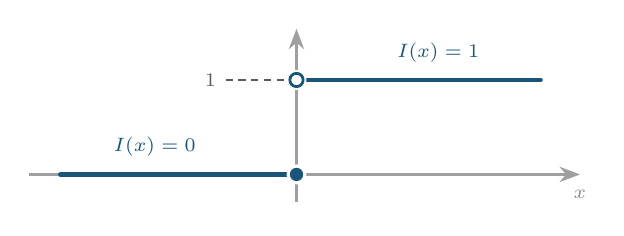
\begin{tikzpicture}[scale=1.0]
    \draw[axisln] (-3.4,0) -- (3.6,0) node[below=2pt, font=\scriptsize,
      gray!90] {$x$};
    \draw[axisln] (0,-0.35) -- (0,1.85);
    \draw[projln, remcolor] (-0.9,1.2) -- (0,1.2);
    \node[remcolor, font=\scriptsize, left] at (-0.9,1.2) {$1$};
    % the graph
    \draw[curveln, defcolor] (-3,0) -- (0,0);
    \draw[curveln, defcolor] (0,1.2) -- (3.1,1.2);
    \dotpt{defcolor}{(0,0)}
    \opendotpt{defcolor}{(0,1.2)}
    \node[defcolor, font=\scriptsize] at (-1.8,0.35) {$I(x) = 0$};
    \node[defcolor, font=\scriptsize] at (1.8,1.55) {$I(x) = 1$};
  \end{tikzpicture}
  \end{center}

  \note{
    We now meet the simplest possible jump. The unit step function
    "I" equals 0 for all "x" less than or equal to 0, and 1 for all
    "x" strictly greater than 0. Look at the graph: the function runs
    along the axis up to and including the origin, where the filled
    blue dot marks the value 0, then jumps to height 1 immediately to
    the right, with the open circle showing that the value 1 is not
    attained at 0 itself. So "I" is continuous from the left at 0 and
    jumps as soon as we move right. Shifting the jump to a point "s"
    by writing "I" of "x" minus "s" gives an increasing weight
    function whose entire growth happens at "s". What does
    integration against such a weight do? The next theorem gives a
    beautiful answer.
  }
\end{frame}

\begin{frame}{Theorem 6.15: Integration Against a Single Jump}
  \begin{thmblock}{Theorem 6.15}
    If $a < s < b$, $f$ is bounded on $[a,b]$, $f$ is
    \alert{continuous at $s$}, and $\alpha(x) = I(x - s)$, then
    \[
      \int_a^b f\,d\alpha = f(s).
    \]
  \end{thmblock}

  \vspace{0.3em}
  \begin{hlbox}
  \textbf{Key idea:} all the weight sits at $s$ --- the integral
  \alert{samples} $f$ there. \quad (Physicists: this is the
  ``$\delta$-function'' made rigorous.)
  \end{hlbox}

  \note{
    Theorem 6.15. Take the weight alpha of "x" equal to "I" of "x"
    minus "s": a single unit jump at the interior point "s". If "f"
    is bounded and continuous at "s", then the Stieltjes integral of
    "f" with respect to this weight is simply "f" of "s". Think of
    the weight as measuring importance: this alpha assigns no
    importance to any part of the interval except the single point
    "s", so the integral ignores everything except the value of "f"
    there. Readers who have met the Dirac delta in physics should
    recognize this: integrating against a point mass samples the
    function, and the Stieltjes framework makes that rigorous with no
    new machinery. The proof takes four partition points.
  }
\end{frame}

\begin{frame}{Proof of Theorem 6.15 --- Only One Interval Counts}
  \begin{proofblock}{A four-point partition}
    Consider $P = \{x_0, x_1, x_2, x_3\}$ with
    $x_0 = a$, \ $x_1 = s < x_2 < x_3 = b$. The increments of
    $\alpha(x) = I(x-s)$:
    \[
      \Delta\alpha_1 = 0, \qquad
      \Delta\alpha_2 = 1, \qquad
      \Delta\alpha_3 = 0.
    \]
    Hence
    \[
      U(P,f,\alpha) = M_2, \qquad L(P,f,\alpha) = m_2.
    \]
  \end{proofblock}

  \begin{center}
  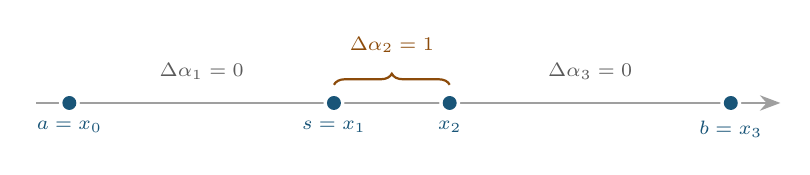
\begin{tikzpicture}[scale=1.05]
    \draw[axisln] (-0.4,0) -- (8.6,0);
    \foreach \x/\lab in {0/{a = x_0}, 3.2/{s = x_1}, 4.6/{x_2},
      8/{b = x_3}} {
      \dotpt{defcolor}{(\x,0)}
      \node[defcolor, font=\scriptsize, below=3pt] at (\x,0) {$\lab$};
    }
    \node[remcolor, font=\scriptsize, above=5pt] at (1.6,0)
      {$\Delta\alpha_1 = 0$};
    \node[excolor, font=\scriptsize, above=5pt] at (3.9,0.32)
      {$\Delta\alpha_2 = 1$};
    \node[remcolor, font=\scriptsize, above=5pt] at (6.3,0)
      {$\Delta\alpha_3 = 0$};
    \draw[decorate,decoration={brace,amplitude=4pt},thick,excolor]
      (3.2,0.22) -- (4.6,0.22);
  \end{tikzpicture}
  \end{center}

  \note{
    Consider very special partitions with only four points: "a"
    itself, then "x" sub 1 equal to the jump point "s", then a point
    "x" sub 2 slightly to the right of "s", then "b". Compute the
    increments of alpha, shown on the number line. From "a" to "s"
    the weight is constantly 0, so the first increment vanishes.
    From "s" to "x" sub 2 the weight rises from 0 to 1, so the middle
    increment is exactly 1; the orange brace marks this interval,
    the only one that carries weight. From "x" sub 2 to "b" the
    weight is constantly 1, so the last increment vanishes too. The
    upper and lower sums collapse to a single term each: the upper
    sum is capital "M" sub 2, the supremum of "f" on the middle
    interval, and the lower sum is lowercase "m" sub 2, the infimum
    there. Now squeeze that middle interval.
  }
\end{frame}

\begin{frame}{Proof of Theorem 6.15 --- Shrink the Interval}
  \begin{proofblock}{Let $x_2 \to s$}
    $f$ is continuous at $s$, so
    \[
      M_2 = \sup_{[s,\,x_2]} f \;\longrightarrow\; f(s)
      \qquad\text{and}\qquad
      m_2 = \inf_{[s,\,x_2]} f \;\longrightarrow\; f(s)
      \qquad (x_2 \to s).
    \]
    Since $L(P,f,\alpha) \leq \underline{\int} f\,d\alpha \leq
    \overline{\int} f\,d\alpha \leq U(P,f,\alpha)$ for these $P$:
    \[
      \boxed{\;\int_a^b f\,d\alpha = f(s).\;} \qed
    \]
  \end{proofblock}

  \note{
    Here is where continuity at "s" earns its keep. As "x" sub 2
    slides down to "s", the middle interval shrinks onto the single
    point "s", and because "f" is continuous there, both the supremum
    and the infimum of "f" over that interval converge to "f" of "s".
    So we have found partitions whose upper and lower sums are both
    as close to "f" of "s" as we like. The lower and upper integrals
    are trapped between them, so both equal "f" of "s", which means
    "f" is integrable with respect to alpha and the integral equals
    "f" of "s". One jump samples one value. The natural next move is
    to pile up infinitely many jumps.
  }
\end{frame}

\begin{frame}{Theorem 6.16: A Series Is an Integral}
  \begin{thmblock}{Theorem 6.16}
    Suppose $c_n \geq 0$, $\sum c_n$ converges, $\{s_n\}$ is a
    sequence of \alert{distinct} points in $(a,b)$, and
    \begin{equation}
      \alpha(x) = \sum_{n=1}^{\infty} c_n\, I(x - s_n). \tag{22}
    \end{equation}
    Let $f$ be continuous on $[a,b]$. Then
    \begin{equation}
      \int_a^b f\,d\alpha = \sum_{n=1}^{\infty} c_n\, f(s_n). \tag{23}
    \end{equation}
  \end{thmblock}

  \vspace{0.3em}
  \begin{hlbox}
  \textbf{Key idea:} a \alert{series} is a Stieltjes
  integral against a pure step function.
  \end{hlbox}

  \note{
    Theorem 6.16 is the showpiece of this section. Build a weight
    function by superposing infinitely many steps: at each point "s"
    sub "n" of a sequence of distinct points, place a jump of
    nonnegative size "c" sub "n", where the series of the "c" sub
    "n" converges. Equation 22 defines this weight. Then for every
    continuous "f", equation 23 says the integral of "f" with respect
    to alpha is the series: sum over "n" of "c" sub "n" times "f" of
    "s" sub "n". Each jump samples "f" at its location, weighted by
    the jump size, and the samples add up. Read backwards, any
    convergent series of this form is an integral, so theorems about
    integrals become theorems about series for free. Here is the
    proof plan.
  }
\end{frame}

\begin{frame}[c]{The Picture: A Staircase Weight}
  \begin{center}
  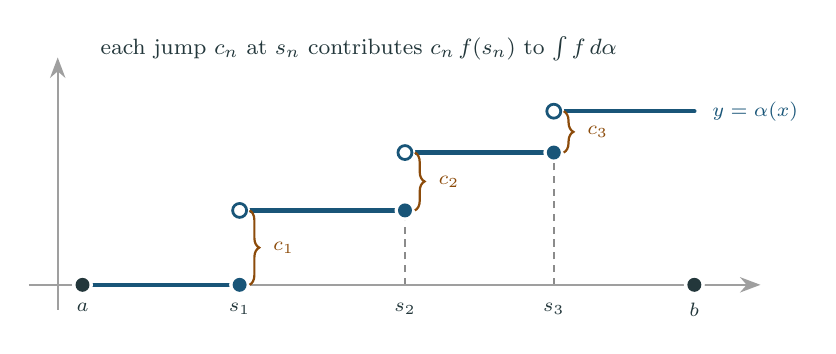
\begin{tikzpicture}[scale=1.05]
    % dashed guides at the jump points
    \foreach \x/\ylo/\yhi in {2.2/0/0.9, 4.2/0.9/1.6, 6.0/1.6/2.1} {
      \draw[projln, remcolor!70] (\x,0) -- (\x,\ylo);
    }
    % axes
    \draw[axisln] (-0.35,0) -- (8.5,0);
    \draw[axisln] (0,-0.3) -- (0,2.75);
    % staircase segments (alpha is left-continuous: I(0) = 0)
    \draw[curveln, defcolor] (0.3,0) -- (2.2,0);
    \draw[curveln, defcolor] (2.2,0.9) -- (4.2,0.9);
    \draw[curveln, defcolor] (4.2,1.6) -- (6.0,1.6);
    \draw[curveln, defcolor] (6.0,2.1) -- (7.7,2.1);
    \dotpt{defcolor}{(2.2,0)}
    \opendotpt{defcolor}{(2.2,0.9)}
    \dotpt{defcolor}{(4.2,0.9)}
    \opendotpt{defcolor}{(4.2,1.6)}
    \dotpt{defcolor}{(6.0,1.6)}
    \opendotpt{defcolor}{(6.0,2.1)}
    % jump-size braces
    \draw[decorate,decoration={brace,amplitude=3.5pt},thick,excolor]
      (2.32,0.9) -- (2.32,0);
    \node[excolor, font=\scriptsize, right=5pt] at (2.32,0.45) {$c_1$};
    \draw[decorate,decoration={brace,amplitude=3.5pt},thick,excolor]
      (4.32,1.6) -- (4.32,0.9);
    \node[excolor, font=\scriptsize, right=5pt] at (4.32,1.25) {$c_2$};
    \draw[decorate,decoration={brace,amplitude=3.5pt},thick,excolor]
      (6.12,2.1) -- (6.12,1.6);
    \node[excolor, font=\scriptsize, right=5pt] at (6.12,1.85) {$c_3$};
    % x labels
    \foreach \x/\lab in {0.3/{a}, 2.2/{s_1}, 4.2/{s_2}, 6.0/{s_3},
      7.7/{b}} {
      \node[mDarkTeal, font=\scriptsize, below=3pt] at (\x,0) {$\lab$};
    }
    \dotpt{mDarkTeal}{(0.3,0)}
    \dotpt{mDarkTeal}{(7.7,0)}
    % curve label
    \node[defcolor, font=\scriptsize, right] at (7.8,2.1)
      {$y = \alpha(x)$};
    % message
    \node[mDarkTeal, font=\footnotesize, align=left, anchor=west]
      at (0.4,2.85)
      {each jump $c_n$ at $s_n$ contributes
       $\alert{c_n\,f(s_n)}$ to $\int f\,d\alpha$};
  \end{tikzpicture}
  \end{center}

  \note{
    Here is what the weight of Theorem 6.16 looks like. The blue
    graph is alpha: a staircase that starts at height 0 at the point
    "a" and climbs by "c" sub 1 at "s" sub 1, by "c" sub 2 at "s"
    sub 2, and by "c" sub 3 at "s" sub 3; the orange braces mark the
    three jump sizes. The dots record a subtlety: at each jump
    point, the filled dot sits on the lower step and the open circle
    on the upper one, because the unit step "I" of 0 is 0, so alpha
    is continuous from the left and jumps just after each "s" sub
    "n". In the real theorem there are infinitely many such jumps,
    with total height the sum of the "c" sub "n". Between jumps
    alpha is flat, so those stretches contribute nothing; as the
    caption says, each jump contributes its size times the value of
    "f" at that point. Now let's turn this picture into a proof.
  }
\end{frame}

\begin{frame}{Proof Strategy: Theorem 6.16}
  \begin{hlbox}
  \textbf{Goal:} $\displaystyle\int_a^b f\,d\alpha
  = \sum_{n=1}^{\infty} c_n f(s_n)$.

  \vspace{0.6em}
  \textbf{Approach:} split the weight, use what we know, let the
  tail vanish.
  \begin{enumerate}
    \item Check $\alpha$ is well defined, increasing, with
      $\alpha(b) - \alpha(a) = \sum c_n$.
    \item Split $\alpha = \alpha_1 + \alpha_2$: the \alert{first $N$
      jumps} plus a \alert{small tail}.
    \item Finite part: Theorems 6.12(e) $+$ 6.15 $\Rightarrow$ a
      finite sum.
    \item Tail: total weight $< \varepsilon$, so Theorem 6.12(d)
      kills it.
    \item Let $N \to \infty$.
  \end{enumerate}
  \end{hlbox}

  \note{
    Before the formal proof, the strategy. Step 1 checks that the
    infinite superposition of steps makes sense and is an increasing
    function whose total rise is the sum of the series. Step 2 is
    the heart: split the weight into the sum of its first "N" jumps,
    a pure step function with finitely many steps, plus the tail
    consisting of all the remaining jumps. Step 3 handles the finite
    part: by linearity in the weight, part "e" of Theorem 6.12,
    together with the one-jump Theorem 6.15, its integral is exactly
    the partial sum of the series. Step 4 handles the tail: its total
    rise is tiny, so the size bound, part "d", makes its integral
    negligible. Step 5 lets "N" go to infinity. Now let's execute.
  }
\end{frame}

\begin{frame}{Proof of Theorem 6.16 --- Step 1: Split the Weight}
  \begin{proofblock}{Step 1: Setup and splitting}
    Comparison test: (22) converges for every $x$;\\
    $\alpha$ is monotonic with $\alpha(a) = 0$, \ $\alpha(b) = \sum c_n$.

    \vspace{0.3em}
    Given $\varepsilon > 0$, choose $N$ with
    $\displaystyle\sum_{N+1}^{\infty} c_n < \varepsilon$, and put
    \[
      \alpha_1(x) = \sum_{n=1}^{N} c_n\,I(x - s_n),
      \qquad
      \alpha_2(x) = \sum_{n=N+1}^{\infty} c_n\,I(x - s_n).
    \]
  \end{proofblock}

  \note{
    First the housekeeping. For each fixed "x", the terms of the
    series 22 are at most "c" sub "n", so the comparison test gives
    convergence, and alpha is well defined. Each summand is an
    increasing function of "x", so alpha is increasing. At "x" equal
    to "a", every step is still switched off, so alpha of "a" is 0;
    at "x" equal to "b", every step has switched on, so alpha of "b"
    is the full sum of the "c" sub "n". Now let epsilon be positive.
    Since the series converges, its tail beyond some index "N" adds
    up to less than epsilon. Split alpha accordingly: alpha sub 1
    carries the first "N" jumps, alpha sub 2 carries all the rest.
    Each piece is increasing, and alpha is their sum.
  }
\end{frame}

\begin{frame}{Proof of Theorem 6.16 --- Step 2: Finite Part and Tail}
  \begin{proofblock}{Step 2: Integrate each piece}
    By Theorems 6.12(e) and 6.15 (applied $N$ times),
    \begin{equation}
      \int_a^b f\,d\alpha_1 = \sum_{n=1}^{N} c_n f(s_n). \tag{24}
    \end{equation}
    Since $\alpha_2(b) - \alpha_2(a) < \varepsilon$, Theorem 6.12(d)
    gives
    \begin{equation}
      \left|\int_a^b f\,d\alpha_2\right| \leq M\varepsilon,
      \qquad M = \sup|f(x)|. \tag{25}
    \end{equation}
  \end{proofblock}

  \note{
    Now integrate against each piece. The weight alpha sub 1 is a
    finite sum of scaled unit steps, so by linearity in the weight,
    part "e" of Theorem 6.12, its integral splits into "N" one-jump
    integrals, and Theorem 6.15 evaluates each: the jump at "s" sub
    "n" of size "c" sub "n" contributes "c" sub "n" times "f" of "s"
    sub "n". That is equation 24: the integral against alpha sub 1
    is exactly the partial sum of the first "N" terms of our target
    series. As for
    the tail weight alpha sub 2, its total rise from "a" to "b" is
    the tail of the series, less than epsilon. The size bound, part
    "d", then says the integral against alpha sub 2 is at most "M"
    epsilon in absolute value, where "M" bounds the absolute value of "f".
    Continuous functions on closed intervals are bounded, so "M" is
    finite. Now assemble.
  }
\end{frame}

\begin{frame}{Proof of Theorem 6.16 --- Step 3: Let $N \to \infty$}
  \begin{proofblock}{Step 3: Assemble and pass to the limit}
    Since $\alpha = \alpha_1 + \alpha_2$, (24) and (25) give
    \begin{equation}
      \left|\int_a^b f\,d\alpha - \sum_{n=1}^{N} c_n f(s_n)\right|
      \leq M\varepsilon. \tag{26}
    \end{equation}
    Let $N \to \infty$: the partial sums converge to the series, and
    (23) follows. \qed
  \end{proofblock}

  \vspace{0.3em}
  \hl{$\boxed{\displaystyle\int_a^b f\,d\alpha
    = \sum_{n=1}^{\infty} c_n\,f(s_n)}$ \quad --- series
  \alert{are} integrals.}

  \note{
    Assembling is one application of linearity in the weight: alpha
    is alpha sub 1 plus alpha sub 2, so the integral against alpha is
    the integral against alpha sub 1, which is the partial sum by
    equation 24, plus the integral against alpha sub 2, which is at
    most "M" epsilon in size by 25. That is inequality 26: the
    integral differs from the partial sum of the first "N" terms by
    at most "M" epsilon. Now recall how "N" was chosen: driving
    epsilon down to zero forces "N" up, so the right hand side of 26
    can be made as small as we please. The partial sums therefore
    converge to the integral. But by definition they converge to the
    series, and a sequence has only one limit, so the integral equals
    the series. Equation 23 is proved. Next we ask the opposite question: what
    if the weight is smooth rather than jumpy?
  }
\end{frame}

}

{
\usebackgroundtemplate{%
  
\includegraphics[width=\paperwidth,height=\paperheight,keepaspectratio=false]{chapter_06_bg_05.png}%
}
\section{Reducing to the Riemann Integral}

\begin{frame}{Theorem 6.17: When the Weight Has a Derivative}
  \begin{thmblock}{Theorem 6.17}
    Assume $\alpha$ increases monotonically and
    $\alpha' \in \mathscr{R}$ on $[a,b]$. Let $f$ be a bounded real
    function on $[a,b]$. Then $f \in \mathscr{R}(\alpha)$
    \alert{if and only if} $f\alpha' \in \mathscr{R}$. In that case
    \begin{equation}
      \int_a^b f\,d\alpha = \int_a^b f(x)\,\alpha'(x)\,dx. \tag{27}
    \end{equation}
  \end{thmblock}

  \vspace{0.3em}
  \begin{hlbox}
  \textbf{Key idea:} \ $d\alpha = \alpha'(x)\,dx$ --- the familiar
  substitution rule.
  \end{hlbox}

  \note{
    Theorem 6.17 is the smooth counterpart of the step function
    theorems. Suppose the increasing weight alpha has a derivative,
    and that derivative is itself Riemann integrable. Then for any
    bounded "f", integrability of "f" with respect to alpha is
    equivalent to ordinary Riemann integrability of the product "f"
    times alpha prime, and when either holds, the two integrals are
    equal; that is equation 27. Symbolically, "d" alpha equals alpha
    prime of "x" "d" "x", the rule everyone learns to manipulate in
    calculus, is here promoted from notation to theorem. Note the
    result is an if and only if, and neither continuity of "f" nor of
    alpha prime is assumed, only integrability of alpha prime. Here
    is the plan of attack.
  }
\end{frame}

\begin{frame}{Proof Strategy: Theorem 6.17}
  \begin{hlbox}
  \textbf{Goal:} show the upper integrals of $f\,d\alpha$ and of
  $f\alpha'\,dx$ \alert{coincide} (then do the same for lower).

  \vspace{0.6em}
  \textbf{Approach:}
  \begin{enumerate}
    \item Apply Theorem 6.6 to $\alpha'$: get $P$ with
      $U(P,\alpha') - L(P,\alpha') < \varepsilon$.
    \item \alert{Mean value theorem}: $\Delta\alpha_i =
      \alpha'(t_i)\,\Delta x_i$ for some $t_i$ in each subinterval.
    \item Theorem 6.7(b): swapping $t_i$ for any $s_i$ costs less
      than $\varepsilon$.
    \item Conclude the two kinds of Riemann sums differ by
      $\leq M\varepsilon$; pass to upper sums, then refinements,
      then upper integrals.
  \end{enumerate}
  \end{hlbox}

  \note{
    The proof is the most technical of this episode, so let's fix the
    road map. The bridge between the two integrals is the mean value
    theorem from Chapter 5: on each subinterval, the rise of alpha
    equals alpha prime evaluated at some intermediate point "t" sub
    "i", times the length of the subinterval. That converts a
    Stieltjes sum for "f" "d" alpha into a Riemann sum for "f" alpha
    prime, except that the sample points for alpha prime are the
    special points "t" sub "i" rather than arbitrary ones. Step 1
    chooses a partition where alpha prime is well controlled, and
    step 3 uses part "b" of Theorem 6.7 to show that moving the
    sample points costs less than epsilon. Step 4 upgrades sums to
    upper integrals. Let's carry it out.
  }
\end{frame}

\begin{frame}{Proof of Theorem 6.17 --- Step 1: Control $\alpha'$}
  \begin{proofblock}{Step 1: A good partition for $\alpha'$, then MVT}
    \small
    Given $\varepsilon > 0$, Theorem 6.6 (applied to $\alpha'$) gives
    a partition $P = \{x_0, \dots, x_n\}$ with
    \begin{equation}
      U(P, \alpha') - L(P, \alpha') < \varepsilon. \tag{28}
    \end{equation}
    The \alert{mean value theorem} furnishes $t_i \in [x_{i-1}, x_i]$
    with
    \[
      \Delta\alpha_i = \alpha'(t_i)\,\Delta x_i \qquad (i = 1, \dots, n).
    \]
    If $s_i \in [x_{i-1}, x_i]$, then by (28) and Theorem 6.7(b),
    \begin{equation}
      \sum_{i=1}^{n} |\alpha'(s_i) - \alpha'(t_i)|\,\Delta x_i
      < \varepsilon. \tag{29}
    \end{equation}
  \end{proofblock}

  \note{
    Step 1. Since alpha prime is Riemann integrable, Theorem 6.6
    provides a partition "P" for which the upper and lower sums of
    alpha prime, with respect to the ordinary length weight, differ
    by less than epsilon; that is 28. On each subinterval, alpha is
    differentiable, so the mean value theorem gives a point "t" sub
    "i" where the derivative matches the average slope: the rise of
    alpha across the subinterval equals alpha prime of "t" sub "i"
    times delta "x" sub "i". This is the exact link between the two
    worlds. Then inequality 29 comes from part "b" of Theorem 6.7,
    applied to alpha prime: whenever a partition satisfies 28,
    sampling alpha prime at any other points "s" sub "i" changes the
    weighted sums by less than epsilon in total.
  }
\end{frame}

\begin{frame}{Proof of Theorem 6.17 --- Step 2: Compare the Two Sums}
  \begin{proofblock}{Step 2: Stieltjes sums vs.\ Riemann sums}
    \small
    Put $M = \sup|f(x)|$. The MVT relation gives
    \[
      \sum_{i=1}^{n} f(s_i)\,\Delta\alpha_i
      = \sum_{i=1}^{n} f(s_i)\,\alpha'(t_i)\,\Delta x_i,
    \]
    so (29) implies
    \begin{equation}
      \left|\sum_{i=1}^{n} f(s_i)\,\Delta\alpha_i
      - \sum_{i=1}^{n} f(s_i)\,\alpha'(s_i)\,\Delta x_i\right|
      \leq M\varepsilon. \tag{30}
    \end{equation}
  \end{proofblock}

  \vspace{0.2em}
  \hl{\textbf{Same $s_i$ in both sums} --- only $\alpha'$'s argument
  moved.}

  \note{
    Step 2 compares the two kinds of sums directly. Take any sample
    points "s" sub "i". The Stieltjes style sum of "f" of "s" sub
    "i" times delta alpha sub "i" is, by the mean value relation,
    identical to the sum of "f" of "s" sub "i" times alpha prime of
    "t" sub "i" times delta "x" sub "i". We would like alpha prime
    evaluated at "s" sub "i" instead, to get an honest Riemann sum
    for the product "f" alpha prime. The damage from switching "t"
    sub "i" to "s" sub "i" is controlled by inequality 29: each
    switch costs the difference of alpha prime values, weighted by
    delta "x" sub "i", and "f" contributes at most a factor of "M".
    Total damage: at most "M" epsilon. That is inequality 30, and it
    holds for every choice of the points "s" sub "i".
  }
\end{frame}

\begin{frame}{Proof of Theorem 6.17 --- Step 3: Upper Sums Are Close}
  \begin{proofblock}{Step 3: From sums to upper sums}
    By (30), for \emph{all} choices of $s_i \in [x_{i-1},x_i]$:
    \[
      \sum_{i=1}^{n} f(s_i)\,\Delta\alpha_i
      \leq U(P, f\alpha') + M\varepsilon
      \quad\Longrightarrow\quad
      U(P, f, \alpha) \leq U(P, f\alpha') + M\varepsilon.
    \]
    The same argument gives
    $U(P, f\alpha') \leq U(P, f, \alpha) + M\varepsilon$. Thus
    \begin{equation}
      \bigl|\,U(P, f, \alpha) - U(P, f\alpha')\,\bigr| \leq
      M\varepsilon. \tag{31}
    \end{equation}
  \end{proofblock}

  \note{
    Step 3 converts the sum estimate into an upper sum estimate. Fix
    the partition "P". By 30, every Stieltjes sum with sample points
    "s" sub "i" is at most the corresponding Riemann sum for "f"
    alpha prime plus "M" epsilon, and that Riemann sum is at most the
    upper sum of "f" alpha prime. Now take the supremum over all
    choices of sample points: on each subinterval, "f" of "s" sub
    "i" can be pushed up toward the supremum "M" sub "i" of "f", so
    the Stieltjes sums approach the upper sum "U" of "P", "f",
    alpha. Hence that upper sum obeys the same bound. Running the
    identical argument starting from equation 30 read in the other
    direction bounds the upper sum of "f" alpha prime by that of "f"
    "d" alpha plus "M" epsilon. Together: the two upper sums differ
    by at most "M" epsilon, which is 31.
  }
\end{frame}

\begin{frame}{Proof of Theorem 6.17 --- Step 4: Pass to the Integrals}
  \begin{proofblock}{Step 4: Refine, then squeeze}
    \small
    (28) survives refinement (Theorem 6.7(a)), hence so does (31).
    Taking infima over all refinements:
    \[
      \left|\;\overline{\int_a^b} f\,d\alpha
      - \overline{\int_a^b} f(x)\,\alpha'(x)\,dx\;\right|
      \leq M\varepsilon.
    \]
    But $\varepsilon$ is arbitrary, so
    \begin{equation}
      \overline{\int_a^b} f\,d\alpha
      = \overline{\int_a^b} f(x)\,\alpha'(x)\,dx
      \qquad \text{for \alert{any} bounded } f. \tag{32}
    \end{equation}
    Lower integrals: identical, from (30). The theorem follows. \qed
  \end{proofblock}

  \note{
    Step 4 finishes. If we refine "P", inequality 28 persists, by
    part "a" of Theorem 6.7, and the whole chain of reasoning
    repeats, so 31 persists for every refinement as well. The upper
    integral is the infimum of upper sums, and it is enough to take
    that infimum over refinements of our fixed "P". Since the two
    upper sums travel within "M" epsilon of each other along all
    these partitions, the two upper integrals are within "M" epsilon
    too. Now epsilon was arbitrary, so they are equal: that is
    equation 32, and notice it holds for any bounded "f",
    integrable or not. The same argument applied to lower sums gives
    equality of the lower integrals. Consequently upper equals lower
    for "f" "d" alpha exactly when upper equals lower for "f" alpha
    prime "d" "x": integrability on one side is integrability on
    the other, and the common values agree, which is equation 27.
  }
\end{frame}

}

{
\usebackgroundtemplate{%
  
\includegraphics[width=\paperwidth,height=\paperheight,keepaspectratio=false]{chapter_06_bg_06.png}%
}
\section{Why Stieltjes?}

\begin{frame}{Remark 6.18: One Theory for Series and Integrals}
  \begin{remblock}{Remark 6.18}
    The two preceding theorems show the \alert{generality and
    flexibility} of the Stieltjes process:
    \begin{itemize}
      \item $\alpha$ a \alert{pure step function} $\Rightarrow$ the
        integral is a finite or infinite \alert{series}
      \item $\alpha' \in \mathscr{R}$ $\Rightarrow$ the integral is an
        ordinary \alert{Riemann integral}
    \end{itemize}
    $\Rightarrow$ series and integrals can be studied
    \alert{simultaneously}, not separately.
  \end{remblock}

  \note{
    Let's step back and see what the two bullets on the slide add up
    to. The first records Theorem 6.16: when the weight is a pure step
    function, one that stands still and grows only by jumping, the
    Stieltjes integral is a finite or infinite series. The second
    records Theorem 6.17: when the weight has an integrable
    derivative, the Stieltjes integral is an ordinary Riemann
    integral. One definition covers both discrete
    summation and continuous integration, so any theorem proved for
    Stieltjes integrals is automatically a theorem about series and
    a theorem about integrals at once. And the weight need not be of
    either special type; it can be continuous yet not differentiable,
    mixing both behaviors. Rudin illustrates with a physical example.
  }
\end{frame}

% --- Build 1/2 ---
\begin{frame}{A Physical Example: Moment of Inertia}
  \begin{exblock}{A wire on an axis}
    A straight wire of unit length spins about an axis through one
    endpoint, at right angles to the wire. Let $m(x) =$ mass
    contained in $[0, x]$. The \alert{moment of inertia} is
    \begin{equation}
      \int_0^1 x^2\,dm. \tag{33}
    \end{equation}
  \end{exblock}

  \note{
    Here is the example. A straight wire of unit length rotates about
    an axis through one of its endpoints, perpendicular to the wire.
    In mechanics, the moment of inertia measures resistance to
    rotation, and each bit of mass contributes its distance from the
    axis squared, times its mass. Describe the mass by the function
    "m", where "m" of "x" is the total mass sitting in the interval
    from 0 to "x". Mass never decreases as the interval grows, so
    "m" is monotonically increasing: a legitimate Stieltjes weight.
    Formula 33 expresses the moment of inertia as the Stieltjes
    integral of "x" squared with respect to "m": distance squared,
    weighted by where the mass actually sits. Now watch this single
    formula specialize in two opposite directions.
  }
\end{frame}

% --- Build 2/2 ---
\begin{frame}{A Physical Example: Moment of Inertia}
  \begin{exblock}{A wire on an axis}
    A straight wire of unit length spins about an axis through one
    endpoint, at right angles to the wire. Let $m(x) =$ mass
    contained in $[0, x]$. The \alert{moment of inertia} is
    \begin{equation}
      \int_0^1 x^2\,dm. \tag{33}
    \end{equation}
  \end{exblock}

  \vspace{-0.2em}
  \begin{columns}[T]
    \begin{column}{0.48\textwidth}
      \centering
      \begin{hlbox}
      \centering
      \textbf{Continuous density} $m' = \rho$:
      \begin{equation}
        \int_0^1 x^2 \rho(x)\,dx \tag{34}
      \end{equation}
      \end{hlbox}

      \vspace{-0.4em}
      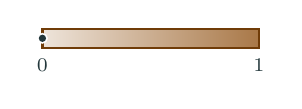
\begin{tikzpicture}[scale=0.55]
        \shade[left color=excolor!15, right color=excolor!75]
          (0,-0.22) rectangle (5,0.22);
        \draw[excolor!80!black, line width=0.8pt]
          (0,-0.22) rectangle (5,0.22);
        \dotpt{mDarkTeal}{(0,0)}
        \node[mDarkTeal, font=\scriptsize, below=4pt] at (0,0) {$0$};
        \node[mDarkTeal, font=\scriptsize, below=4pt] at (5,0) {$1$};
      \end{tikzpicture}
    \end{column}
    \begin{column}{0.48\textwidth}
      \centering
      \begin{hlbox}
      \centering
      \textbf{Point masses} $m_i$ at $x_i$:
      \begin{equation}
        \sum_i x_i^2\, m_i \tag{35}
      \end{equation}
      \end{hlbox}

      \vspace{-0.4em}
      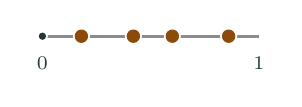
\begin{tikzpicture}[scale=0.55]
        \draw[remcolor!70, line width=1.1pt] (0,0) -- (5,0);
        \foreach \x in {0.9, 2.1, 3.0, 4.3} {
          \fill[white] (\x,0) circle (5.6pt);
          \fill[excolor] (\x,0) circle (4.4pt);
        }
        \dotpt{mDarkTeal}{(0,0)}
        \node[mDarkTeal, font=\scriptsize, below=4pt] at (0,0) {$0$};
        \node[mDarkTeal, font=\scriptsize, below=4pt] at (5,0) {$1$};
      \end{tikzpicture}
    \end{column}
  \end{columns}

  \note{
    On the left, suppose the wire has a continuous density rho, so
    that "m" prime equals rho; the shading of the bar suggests the
    mass thickening toward the right end. Theorem 6.17 turns formula
    33 into formula 34, the ordinary Riemann integral of "x" squared
    times rho of "x". On the right, suppose instead the wire is
    massless except for beads of mass "m" sub "i" concentrated at
    the points "x" sub "i", drawn as orange dots. Then "m" is a pure
    step function, and Theorem 6.16 turns 33 into 35, the finite sum
    of "x" sub "i" squared times "m" sub "i". One physical
    quantity, one formula, and the Stieltjes integral handles the
    continuous wire, the beaded wire, and even a wire whose mass
    function is continuous yet has no derivative, all at once, with no
    change to formula 33. One more theorem completes our toolkit: change of
    variable.
  }
\end{frame}

}

{
\usebackgroundtemplate{%
  
\includegraphics[width=\paperwidth,height=\paperheight,keepaspectratio=false]{chapter_06_bg_07.png}%
}
\section{Change of Variable}

\begin{frame}{Theorem 6.19: Change of Variable}
  \begin{thmblock}{Theorem 6.19}
    Suppose $\varphi$ is a \alert{strictly increasing continuous}
    function mapping $[A,B]$ \emph{onto} $[a,b]$. Suppose $\alpha$
    increases monotonically on $[a,b]$ and $f \in \mathscr{R}(\alpha)$
    on $[a,b]$. Define $\beta$ and $g$ on $[A,B]$ by
    \begin{equation}
      \beta(y) = \alpha(\varphi(y)), \qquad
      g(y) = f(\varphi(y)). \tag{36}
    \end{equation}
    Then $g \in \mathscr{R}(\beta)$ and
    \begin{equation}
      \int_A^B g\,d\beta = \int_a^b f\,d\alpha. \tag{37}
    \end{equation}
  \end{thmblock}

  \note{
    The last theorem of this episode is the change of variable
    formula, in a remarkably clean form. Let phi be a strictly
    increasing continuous map from the interval capital "A" to
    capital "B" onto the interval "a" to "b"; think of it as a
    relabeling of
    the points, possibly stretching here and compressing there. Pull
    everything back through phi: the new weight beta is alpha
    composed with phi, and the new integrand "g" is "f" composed
    with phi, as in equation 36. Then "g" is integrable with respect
    to beta, and the two integrals in 37 are equal. Notice what is
    absent: no differentiability of phi, no derivative factor in the
    formula. The weight absorbs all the distortion. The proof is
    almost pure bookkeeping.
  }
\end{frame}

\begin{frame}{Proof of Theorem 6.19 --- Partitions Correspond}
  \begin{proofblock}{Proof}
    \footnotesize
    Partitions $P = \{x_0, \dots, x_n\}$ of $[a,b]$ correspond to
    partitions $Q = \{y_0, \dots, y_n\}$ of $[A,B]$ via
    $x_i = \varphi(y_i)$ --- \alert{all} of them arise this way.
    $f$ on $[x_{i-1},x_i]$ takes the \alert{same values} as $g$ on
    $[y_{i-1},y_i]$, so
    \begin{equation}
      U(Q,g,\beta) = U(P,f,\alpha), \qquad
      L(Q,g,\beta) = L(P,f,\alpha). \tag{38}
    \end{equation}
    Choose $P$ making both close to $\int f\,d\alpha$ (Theorem 6.6);\\
    Then (38) gives $g \in \mathscr{R}(\beta)$ and (37). \qed
  \end{proofblock}

  \begin{center}
  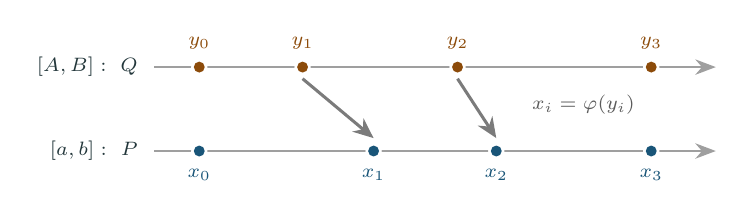
\begin{tikzpicture}[scale=0.82]
    \draw[axisln] (-0.3,1.3) -- (8.4,1.3);
    \node[font=\scriptsize, mDarkTeal, left] at (-0.4,1.3)
      {$[A,B]:\ Q$};
    \foreach \x/\lab in {0.4/{y_0}, 2.0/{y_1}, 4.4/{y_2}, 7.4/{y_3}} {
      \dotpt{excolor}{(\x,1.3)}
      \node[excolor, font=\scriptsize, above=3pt] at (\x,1.3) {$\lab$};
    }
    \draw[axisln] (-0.3,0) -- (8.4,0);
    \node[font=\scriptsize, mDarkTeal, left] at (-0.4,0)
      {$[a,b]:\ P$};
    \foreach \x/\lab in {0.4/{x_0}, 3.1/{x_1}, 5.0/{x_2}, 7.4/{x_3}} {
      \dotpt{defcolor}{(\x,0)}
      \node[defcolor, font=\scriptsize, below=3pt] at (\x,0) {$\lab$};
    }
    \draw[guide, remcolor!80] (2.0,1.12) -- (3.1,0.2);
    \draw[guide, remcolor!80] (4.4,1.12) -- (5.0,0.2);
    \node[remcolor, font=\scriptsize] at (6.35,0.72)
      {$x_i = \varphi(y_i)$};
  \end{tikzpicture}
  \end{center}

  \note{
    Here is the whole proof in one picture. On the bottom line, a
    partition "P" of the interval from "a" to "b" with blue points;
    on the top line, the corresponding partition "Q" of the interval
    from capital "A" to capital "B" with orange points; the gray
    arrows show phi carrying "y" sub "i" to "x" sub "i". Because phi
    is strictly increasing, continuous, and onto, this correspondence
    between partitions is perfect: every partition on one side comes
    from exactly one on the other. Moreover "f" on subinterval
    number "i" downstairs runs through exactly the same values as
    "g" on subinterval number "i" upstairs, and the weight increments
    match: beta of "y" sub "i" equals alpha of "x" sub "i". So upper
    sums equal upper sums and lower sums equal lower sums; that is
    equation 38. Choosing "P" so that both sums hug the integral of
    "f", Theorem 6.6 delivers integrability of "g" and equality of
    the integrals.
  }
\end{frame}

\begin{frame}{The Classical Substitution Rule}
  \begin{exblock}{Special case of (37)}
    Take $\alpha(x) = x$. Then $\beta = \varphi$. Assume
    $\varphi' \in \mathscr{R}$ on $[A,B]$. Applying Theorem 6.17 to
    the left side of (37):
    \begin{equation}
      \int_a^b f(x)\,dx
      = \int_A^B f(\varphi(y))\,\varphi'(y)\,dy. \tag{39}
    \end{equation}
  \end{exblock}

  \vspace{0.3em}
  \begin{hlbox}
  \textbf{The calculus workhorse} ``$u$-substitution'' = Theorem 6.19
  (relabel) $+$ Theorem 6.17 ($d\varphi = \varphi'\,dy$).
  \end{hlbox}

  \note{
    As a dividend, we recover the substitution rule of elementary
    calculus. Take the weight alpha of "x" equal to "x", so the left
    side of 37 is the ordinary integral of "f". Then beta equals phi
    itself, and 37 says this integral equals the Stieltjes integral
    of "f" composed with phi, with respect to phi. If phi happens
    to have an integrable derivative, Theorem 6.17 converts that
    Stieltjes integral into the ordinary integral of "f" of phi of
    "y" times phi prime of "y". Equation 39 is exactly the formula
    used in every substitution: the change of variable rule is the
    composition of two Stieltjes facts, relabeling the interval,
    then trading "d" phi for phi prime "d" "y". Time to sum up the
    episode.
  }
\end{frame}

}

{
\usebackgroundtemplate{%
  
\includegraphics[width=\paperwidth,height=\paperheight,keepaspectratio=false]{chapter_06_bg_08.png}%
}
\section{Summary}

% --- Build 1/4 ---
\begin{frame}{Summary}
  \begin{hlbox}
  \textbf{Key takeaways from this section:}
  \footnotesize
  \begin{itemize}
    \item \textbf{Theorem 6.12:} the integral is \alert{linear} in
      $f$ \emph{and} in $\alpha$, respects order, splits at any
      $c \in (a,b)$, and obeys
      $\bigl|\int f\,d\alpha\bigr| \leq M[\alpha(b) - \alpha(a)]$
  \end{itemize}
  \end{hlbox}

  \note{
    Let's review what we covered. First, the algebra: Theorem 6.12.
    The integral is linear in the function and, just as usefully,
    linear in the weight. It respects order, so larger functions
    have larger integrals, and every estimate in integration theory
    traces back to that. It splits across any intermediate point,
    the two pieces adding to the whole. And it obeys the basic size
    bound: the integral is at most the bound on the function times
    the total rise of the weight. The proofs all followed one
    pattern: compare sums for a common refinement, then apply the
    Theorem 6.6 criterion. Next, closure.
  }
\end{frame}

% --- Build 2/4 ---
\begin{frame}{Summary}
  \begin{hlbox}
  \textbf{Key takeaways from this section:}
  \footnotesize
  \begin{itemize}
    \item \textbf{Theorem 6.12:} the integral is \alert{linear} in
      $f$ \emph{and} in $\alpha$, respects order, splits at any
      $c \in (a,b)$, and obeys
      $\bigl|\int f\,d\alpha\bigr| \leq M[\alpha(b) - \alpha(a)]$
    \item \textbf{Theorem 6.13:} $fg$ and $|f|$ stay integrable
      (polarization $+$ composition), and
      $\bigl|\int f\,d\alpha\bigr| \leq \int |f|\,d\alpha$
  \end{itemize}
  \end{hlbox}

  \note{
    Second, Theorem 6.13. The integrable functions are closed under
    two more operations: multiplication and absolute value. Both came
    from a single source, the composition theorem 6.11 from last
    episode, used once with "t" squared and once with the absolute
    value of "t", together with the polarization identity that
    rebuilds a product out of squares. The inequality on the slide,
    the absolute value of the integral is at most the integral of the
    absolute value, is the triangle inequality for integrals, and one
    well chosen sign was enough to prove it. Now the step functions.
  }
\end{frame}

% --- Build 3/4 ---
\begin{frame}{Summary}
  \begin{hlbox}
  \textbf{Key takeaways from this section:}
  \footnotesize
  \begin{itemize}
    \item \textbf{Theorem 6.12:} the integral is \alert{linear} in
      $f$ \emph{and} in $\alpha$, respects order, splits at any
      $c \in (a,b)$, and obeys
      $\bigl|\int f\,d\alpha\bigr| \leq M[\alpha(b) - \alpha(a)]$
    \item \textbf{Theorem 6.13:} $fg$ and $|f|$ stay integrable
      (polarization $+$ composition), and
      $\bigl|\int f\,d\alpha\bigr| \leq \int |f|\,d\alpha$
    \item \textbf{Theorems 6.14--6.16:} step-function weights
      \alert{sample} $f$: \ $\int f\,d\alpha = \sum c_n f(s_n)$: \\
      a series \alert{is} an integral
  \end{itemize}
  \end{hlbox}

  \note{
    Third, sampling. The unit step of Definition 6.14 concentrates all
    of its growth at one point, and Theorem 6.15 showed that
    integrating against such a weight simply reads off the value of
    "f" there. Theorem 6.16 then stacked up countably many jumps, and
    the integral turned into the series on the slide: the sum of "c"
    sub "n" times "f" of "s" sub "n". So a convergent series is
    literally a Stieltjes integral, which is the most surprising
    result of the episode. One group of results remains.
  }
\end{frame}

% --- Build 4/4 ---
\begin{frame}{Summary}
  \begin{hlbox}
  \textbf{Key takeaways from this section:}
  \footnotesize
  \begin{itemize}
    \item \textbf{Theorem 6.12:} the integral is \alert{linear} in
      $f$ \emph{and} in $\alpha$, respects order, splits at any
      $c \in (a,b)$, and obeys
      $\bigl|\int f\,d\alpha\bigr| \leq M[\alpha(b) - \alpha(a)]$
    \item \textbf{Theorem 6.13:} $fg$ and $|f|$ stay integrable
      (polarization $+$ composition), and
      $\bigl|\int f\,d\alpha\bigr| \leq \int |f|\,d\alpha$
    \item \textbf{Theorems 6.14--6.16:} step-function weights
      \alert{sample} $f$: \ $\int f\,d\alpha = \sum c_n f(s_n)$: \\
      a series \alert{is} an integral
    \item \textbf{Theorem 6.17:} $\alpha' \in \mathscr{R}
      \Rightarrow d\alpha = \alpha'\,dx$ --- back to Riemann;
      \textbf{6.19:} change of variable, no derivative needed
  \end{itemize}

  \vspace{0.8em}
  \normalsize
  \textbf{Coming up next:} The \alert{Fundamental Theorem of Calculus}.
  \end{hlbox}

  \note{
    Finally, the two reductions. When the weight has an integrable
    derivative, Theorem 6.17 converts the Stieltjes integral into
    the ordinary Riemann integral of "f" times alpha prime, making
    the symbolic rule "d" alpha equals alpha prime "d" "x" a
    theorem. Theorem 6.19 gave a change of variable formula with no
    derivatives at all, and combining the two recovered the
    classical substitution rule. Together with Remark 6.18, the
    message of this episode is that series and integrals are one
    subject. In the next episode the derivative finally meets the
    integral: we prove that integration and differentiation are
    inverse operations, the Fundamental Theorem of Calculus, along
    with integration by parts. See you there.
  }
\end{frame}
}

\end{document}
